% % % % % % % % % % % % % % % % % % % % % % % % % % % % % % % % % % % % % % % % % % % %
%                                                                                     %
% Short Sectioned Assignment LaTeX Template Version 1.0 (5/5/12)                      %
% This template has been downloaded from: http://www.LaTeXTemplates.com               %
%                                                                                     %
% Original author:  Frits Wenneker (http://www.howtotex.com)                          %
%                                                                                     %
% Modified by: Fco Javier Sueza Rodríguez (fcosueza@disroot.org)                      %
%                                                                                     %
% Changes:                                                                            %
%	    - Custom Chapters, Sections and Subsections (titlesec package)                %
%           - Document type scrbook (oneside)                                         %
%           - Use babel-lang-spanish package and marvosym                             %
%           - Use hyperref, enumitem, tcolorbox and glossaries packages               %
%           - Use Time New Roman (mathptmx), Helvetic and Courier fonts               %
%                                                                                     %
% License: CC BY-NC-SA 3.0 (http://creativecommons.org/licenses/by-nc-sa/3.0/)        %
%                                                                                     %
% % % % % % % % % % % % % % % % % % % % % % % % % % % % % % % % % % % % % % % % % % % %

%-----------------------------------------------%
%	              Packages                  %
%-----------------------------------------------%

\documentclass[paper=a4, fontsize=11pt, oneside]{scrbook}

% ---- Text Input/Output ----- %

\usepackage[T1]{fontenc}
\usepackage[utf8]{inputenc}
\usepackage{mathptmx}
\usepackage[scaled=.92]{helvet}
\usepackage{courier}
\usepackage[indent=12pt]{parskip}

\usepackage{geometry}
\geometry{verbose,tmargin=3cm,bmargin=3cm,lmargin=2.6cm,rmargin=2.6cm}

% ---- Language ----- %

\usepackage[spanish]{babel}
\usepackage{marvosym}

% ---- Another packages ---- %

\usepackage{amsmath,amsfonts,amsthm}
\usepackage{graphics,graphicx}
\usepackage{titlesec}
\usepackage{fancyhdr}
\usepackage{tcolorbox}
\usepackage{hyperref}
\usepackage{enumitem}
\usepackage[automake]{glossaries}

%--------------------------------------------------------------------%
%                      Customizing Document                          %
%--------------------------------------------------------------------%


% ----------- Custom Chapters, Sections and Subsections -------------- %

\titleformat{\chapter}[display]
			{\bfseries\Huge}
			{Tema \ \thechapter} {0.5ex}
			{\vspace{1ex}\centering}

\titleformat{\section}[hang]
			{\bfseries\Large}
			{\thesection}{0.5em}{}

\titleformat{\subsection}[hang]
			{\bfseries\large}
			{\thesubsection}{0.5em}{}

\titleformat{\subsubsection}[hang]
			{\bfseries\large}
			{\thesubsubsection}{0.5em}{}

\hypersetup{
    colorlinks=true,
    linkcolor=black,
    urlcolor=magenta
}

% ------------------- Custom heaaders and footers ------------------- %

\pagestyle{fancyplain}

\fancyhead[]{}
\fancyfoot[L]{}
\fancyfoot[C]{}
\fancyfoot[R]{\thepage}

\renewcommand{\headrulewidth}{0pt} % Remove header underlines
\renewcommand{\footrulewidth}{0pt} % Remove footer underlines

\setlength{\headheight}{13.6pt} % Customize the height of the header

% --------- Numbering equations, figures and tables ----------------- %

\numberwithin{equation}{section} % Number equations within sections
\numberwithin{figure}{section} % Number figures within sections
\numberwithin{table}{section} % Number tables within sections

% ------------------------ New Commands ----------------------------- %

\newcommand{\horrule}[1]{\rule{\linewidth}{#1}} % Create horizontal rule command


%----------------------------------------------------------------------------------------
%	TÍTULO Y DATOS DEL ALUMNO
%----------------------------------------------------------------------------------------

\title{
\vspace{10ex}
\normalfont \normalsize
\Huge \textbf{Tarea 2: Sistemas Operativos y Software de un Sistema Informático}
}
\author{Francisco Javier Sueza Rodríguez}
\date{\normalsize\today}

%----------------------------------------------------------------------------------------
%                                     DOCUMENTO
%----------------------------------------------------------------------------------------
\begin{document}

\maketitle

\thispagestyle{empty}

\vspace{68ex}

\begin{center}
    \begin{tabular}{l l}
        \textbf{Centro}: & IES Aguadulce \\
        \textbf{Ciclo Formativo}: & Desarrollo Aplicaciones Web (Distancia)\\
        \textbf{Asignatura}: & Sistemas Informáticos\\
        \textbf{Tema}: & Tema 2 -  Software de un Sistema Informático\\
    \end{tabular}
\end{center}

\newpage

\tableofcontents

\vspace{15ex}

%\hrule

%\vspace{10ex}

%\listoffigures

\newpage

\section{Caso Práctico}
\textbf{Ada}, fundadora de la empresa AguadulSoft, ha visto una oportunidad excepcional de promocionar la empresa aprovechando una exposición temporal denominada "Historia del software: Sistemas Operativos" que se va a alojar en la localidad.

La empresa, a la que se le ha pedido colaboración, realizará un análisis de los distintos Sistemas Operativos así como de otros tipos de software que han surgido a lo largo de la historia.

También va a averiguar qué licencias se utilizan en los sistemas operativos y distintos programas que se utilizan en la actualidad.

\section{Actividades}

\subsection{Actividad  1: Tipos de Aplicaciones Informáticas}
Indica, justificando su uso, dos ejemplos de aplicaciones de propósito general y otros dos de propósito específico para cada uno de los siguientes entornos productivos:

\begin{itemize}
    \item Agencia de Viajes
    \item Agencia de Publicidad y Marketing
\end{itemize}

\subsubsection{Solución}
Estas dos empresas usaran tanto aplicaciones de propósito general como específico de su propio campo. En la siguiente lista se muestran dos ejemplos de cada tipo de software para cada una de las empresas.

\begin{itemize}
    \item \textbf{Agencia de Viajes}
    \begin{itemize}
        \item \textbf{Aplicaciones de Propósito General}
        \begin{itemize}
            \item \textbf{Hoja de Cálculo}: es muy probable que usen hojas de cálculo, ya que los viajes tienen muchos complementos y añadidos, y una hoja de cálculos será necesaria para calcular el precio final del paquete elegido por el cliente. Probablemente usen \textbf{Excel} o alguna alternativa libre como \textbf{Libreoffice Calc} o \textbf{Calc de Openoffice}.

            \item \textbf{Herramientas de Acceso de Bases de Datos}: también deberán emplear alguna herramienta de acceso y gestión de bases de datos, para poder consultar y administrar los destinos disponibles, precios, paquetes, etc...
        \end{itemize}

    \item \textbf{Aplicaciones de Propósito Específico}
    \begin{itemize}
        \item \textbf{Aplicaciones Ad-hoc Especializadas}: para la gestión de la agencia de viajes, los clientes, billetes, comunicación con terceros (hoteles, guías turísticos,..) se utilizará algún \textbf{CRM} especializado, como por ejemplo \textbf{CRM Travel}.

        \item \textbf{Herramientas de Administración de Bases de Datos}: además de un CRM, se deberá usar una bases de datos y herramientas para su administración, ya que este tipo de aplicaciones necesitan una base de datos como soporte. Así, podrá centralizarse toda la información de la empresa y permitirle al CRM hacer una gestión adecuada de toda esta información. Una de estás aplicaciones podría ser \textbf{OracleDB}, una de las más empleadas a nivel mundial, o \textbf{MySQL}, otra de la más usadas también.
    \end{itemize}

    \vspace{5ex}
    \end{itemize}

    \item \textbf{Agencia de Publicidad y Marketing}
    \begin{itemize}
        \item \textbf{Aplicaciones de Propósito General}
        \begin{itemize}
            \item \textbf{Generador de Presentación}: una herramienta necesaria para exponer información será un generador de presentación, bien para presentar la estrategia de una nueva campaña y sus elementos claves o para presentar datos relativos a una campaña ya realizar, entre otras cosas. Podrían usar \textbf{Microsoft Powerpoint}, por ejemplo.

            \item \textbf{Herramientas para la Comunicación}: seguramente también usen herramientas para la comunicación rápida y directa entre los diferentes departamentos, ya que el trabajo de esta empresa debe estar bien coordinado entre los diferentes equipos que conformen un mismo proyecto. Este software podría ser \textbf{Slack}, uno de los más usados.
        \end{itemize}

        \item \textbf{Aplicaciones de Propósito Específico}
        \begin{itemize}
            \item \textbf{Herramientas de Diseño Gráfico y Maquetación}: esta herramienta será básica para el diseño de campañas publicitarias, especialmente aquellas pensadas para cartelería o cualquier medio impreso. Uno de los más usados es \textbf{Adobe Photoshop}, aunque también podrían usar alternativas como libres como \textbf{Gimp} o \textbf{Inkscape}, o incluso usar la herramienta colaborativa \textbf{Figma}, cuyo uso se esta expandiendo recientemente.

            \item \textbf{Herramientas de Análisis de Datos}: la empresa necesitará diferentes herramientas de análisis de datos para conocer el impacto de las campañas, punto clave para saber si han tenido éxito o no. Esto requiere de herramientas que sean capaces de procesar grandes cantidades de datos, conocidas como \textbf{Big Data}. Una de las empleadas es \textbf{HubSpot}, especializada en el análisis de datos de marketing.
        \end{itemize}
    \end{itemize}
\end{itemize}

\subsection{Actividad 2: Licencias de Software}
Indica para cada una de las siguientes aplicaciones, el tipo de licencia que utiliza, intentando dar en términos generales si se trata de una licencia de software con código abierto, con código cerrado o de dominio público (sin licencia), y de manera específica la licencia exacta que utiliza.

Por ejemplo: El programa de edición de gráficos vectoriales llamado Inkscape, usa una licencia GPLv3+, que es una licencia de software con código abierto, no permisiva, de tipo copyleft fuerte (software libre).

Las aplicaciones son las siguientes:

\begin{itemize}
    \item Microsoft Office 2021.
    \item Google Chrome.
    \item VLC Media Player.
    \item Avast Free Antivirus.
    \item Adobe Acrobat Pro.
\end{itemize}

\subsubsection{Solución}
En esta actividad vamos a indicar bajo que licencia están desarrolladas diferentes aplicaciones, especificando si la licencia es libre y propietaria, así como sus principales características.

\begin{itemize}
    \item \textbf{Microsoft Office 2021}: esta suite ofimática se encuentra bajo la licencia \textbf{Microsoft CLUF}, una \textbf{licencia propietaria} de tipo \textbf{EULA}, que no permite distribución del software ni incluye su código fuente, además, solo permite su uso para un único usuario. \cite{mscluf01}

    \item \textbf{Google Chrome}: este navegador se encuentra bajo los \textbf{Términos de Servicio Adicionales de Chrome y Chrome OS} \cite{wiki01}, que establece una \textbf{licencia propiertaria freeware} para los binarios de Google Chrome, que permite su uso de forma gratuita y por tiempo ilimitado.

     En cambio, este navegador esta basado en \textbf{Chromium} \cite{chrome01}, por lo que la mayoría de sus componentes software están bajo la licencia \textbf{3-clause BSD}, una licencia de \textbf{código abierto} de tipo \textbf{permisiva} \cite{wiki02}, que garantiza el uso y distribución del software y su código fuente.

     \item \textbf{VLC Media Player}: este reproductor de vídeo esta bajo una \textbf{licencia de código abierto}, en concreto, esta licencia es la \textbf{GPLv2.1+} \cite{vcl01}, una licencia de tipo \textbf{copyleft fuerte} que garantiza la distribución tanto del software como de su código fuente siempre cuando se conserve la licencia en los productos derivados.

     \item \textbf{Avast Free Antivirus}: la versión gratuita de \textbf{Avast Antivirus} usa una \textbf{licencia propietaria}, la \textbf{Avast EULA}, de tipo \textbf{freeware} y \textbf{EULA}. Su uso es gratuito por tiempo ilimitado para un solo usuario, prohibiendo explícitamente su uso para uso comercial o su uso por parte de cualquier compañía o entidad gubernamental. \cite{avas1}

     \item \textbf{Adobe Acrobat Pro}: los productos de Adobe se rigen por la licencia \textbf{Adobe EULA}, una \textbf{licencia propietaria} de tipo \textbf{EULA}. La licencia tiene dos modalidades, una \textbf{freeware} y otra \textbf{comercial}. En este caso, la versión \textbf{Pro} de Adobe Acrobat usa la modalidad \textbf{comercial}. \cite{adobe1}
\end{itemize}

\subsection{Actividad 3:  Sistemas operativos: Última versión, requisitos hardware,...}
Realiza la siguiente tabla añadiendo una fila por sistema operativo con la última versión existente de:

\begin{itemize}
    \item Windows 11 (canal de disponibilidad general).
    \item Ubuntu Desktop LTS (última versión con soporte de larga duración).
    \item iOS (para iOS, en lugar de "requisitos hardware", incluye una lista con los dispositivos que soportan la última versión).
    \item iOS (para iOS, en lugar de "requisitos hardware", incluye una lista con los dispositivos que soportan la última versión).
\end{itemize}

\begin{figure}[ht]
    \centering
    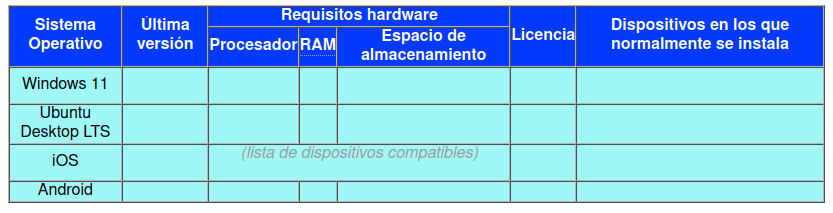
\includegraphics[scale=0.55]{tabla-so.png}
    \caption{Tabla para rellenar sobre SOs}
\end{figure}

\subsubsection{Solución}
En este punto vamos a ver información básica sobre los diferentes sistemas operativos más extendidos en la actualidad. En la siguiente figura se muestra una tabla con toda la información pedida.

Dentro de la sección de requisitos de hardware se incluirán los requisitos mínimos, no los recomendados. El colo de la tabla también puede diferir de la que se muestra en el enunciado, pero el contenido es el solicitado.

\begin{figure}[ht]
    \centering
    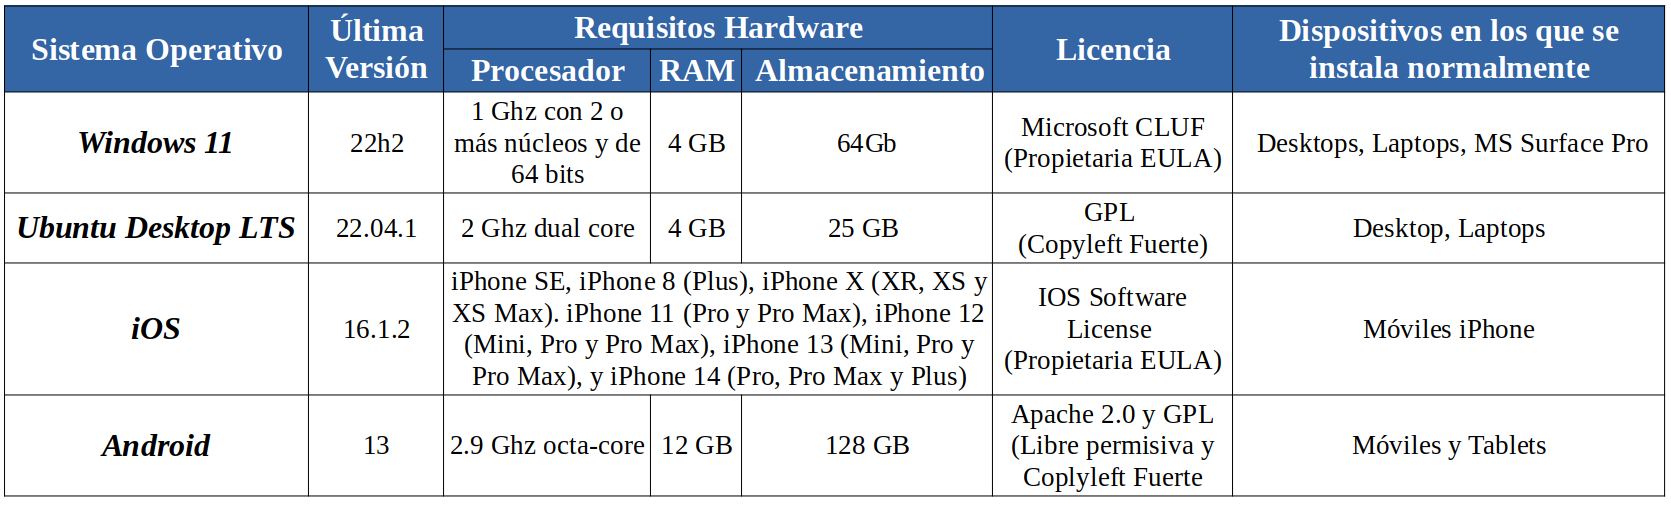
\includegraphics[scale=0.35]{tabla-so-completa.png}
    \caption{Tabla características SOs}
\end{figure}

Para el apartado de \textbf{Android}, se ha incluido el teléfono \textbf{Samsung Galaxy S21 Ultra}. Actualmente no hay móviles que salgan con Android 13, ya que esta versión es muy reciente (Agosto de 2022), pero si hay muchos que se han actualizado a esta versión desde la versión 12, este Samsung es uno de ellos.

\subsection{Actividad 4: Arquitectura Interna de un Sistema Operativo}
Explica en qué consisten las siguientes arquitecturas de sistemas operativos:

\begin{itemize}
    \item Monolítica.
    \item Microkernel.
    \item Híbrida.
\end{itemize}

Indica, además, un ejemplo de SO para cada arquitectura.

\subsubsection{Solución}
En este punto vamos a explicar diferentes arquitecturas de Kernel, explicando un poco sus características y poniendo un ejemplo de un sistema operativo que las use.

\begin{itemize}
    \item \textbf{Arquitectura Monolítica}

    En este tipo de arquitectura \textbf{todas las funciones} se implementan \textbf{dentro del núcleo}, es decir, todos los servicios del sistema operativo se ejecutan dentro de hilo principal del Kernel. También se incluyen dentro del núcleo \textbf{todos los drivers} necesarios para que funcionen los diferentes dispositivos. Este tipo de arquitectura ha sido empleado tradicionalmente por los sistemas tipo Unix. \cite{wiki04}

    Algunos desarrolladores, como Ken Thompson, mantienen que es ``más fácil de implementar'' que otras arquitecturas, como los microkernels, aunque son núcleos más difíciles de mantener, principalmente por la dependencia entre los componentes del sistema. \cite{wiki03}

    Algunos ejemplos de este tipo de kernel son los sistemas \textbf{GNU/Linux}, \textbf{BSD} (FreeBSD, OpenBSD, NetBSD), y los sistemas basados en \textbf{UNIX System V}, como \textbf{Solaris} o \textbf{HP-UX}. El sistema \textbf{MS-DOS} también usaba esta arquitectura.

    \item \textbf{Microkernel}

    En este tipo de arquitectura, muchas de las \textbf{funcionalidades} que históricamente se implementaban dentro del kernel se mueven \textbf{fuera de éste}, en un conjunto de ``\textbf{servidores}'' que se comunican a través de un kernel con el mínimo posible de código. Estos servidores, al contrario que en otros kernel, se ejecutan en el \textbf{espacio de usuario} en vez de en el \textbf{espacio de sistema}, manteniéndose en éste solo lo imprescindible, como el \textbf{IPC} (Inter Process Comunitacion), que permite la comunicación entre los diferentes procesos. \cite{wiki03}

    Esta arquitectura tiene varias \textbf{ventajas} sobre la monolítica, como que son \textbf{más fácil de mantener}, los \textbf{parches} se pueden \textbf{testear} en instancias separadas y son más rápidos de desarrollar. Pero también tiene algunos \textbf{inconvenientes}, como que los \textbf{programas necesitan más memoria} para poder ejecutarse, la \textbf{gestión de procesos} es más \textbf{compleja}, y el rendimiento es menor que en los kernel monolíticos. \cite{wiki03}

    Algunos ejemplos de sistemas operativos con microkernel son \textbf{AmigaOS}, \textbf{Minix} y 	\textbf{HarmonyOS}, entre otros.

    \item \textbf{Arquitectura Híbrida}

    Estos tipos de kernel son \textbf{similares} a los \textbf{microkernel}, con la diferencia de que \textbf{incluyen más funcionalidades} dentro de \textbf{núcleo} para mejorar el rendimiento de éste, combinando, por así decirlo, las arquitecturas monolítica y microkernel. La idea es tener una estructura similar a un microkernel, pero implementando esa estructura de forma monolítica, así, no tienen los beneficios de tener los servicios del SO en el espacio de usuario, pero tampoco tienen la sobrecarga en el paso de mensajes que esto puede ocasionar, siendo en este aspecto más similar a un kernel monolítico. \cite{wiki05}

    El ejemplo más conocido de este tipo de kernel son los sistemas \textbf{Microsoft Windows}, que desde la versión \textbf{Windows NT} se lleva empleando en todos sus sistemas operativos, incluido la ultima versión, \textbf{Windows 11}. También hay otros sistemas que emplean este tipo de arquitectura, como \textbf{BeOS}, \textbf{Netware} o \textbf{ReactOS}.
\end{itemize}

\subsection{Actividad 5: Gestión de Procesos}
Sabemos las siguientes características sobre un sistema operativo:

\begin{enumerate}
    \item Utiliza el algoritmo de planificación de procesos SJF (el trabajo más corto primero), el cual es un algoritmo no apropiativo.
    \item Necesita ejecutar una serie de procesos, cuyos instantes de llegada y tiempos que tardan en ejecutarse se representan en la siguiente tabla:

    \begin{figure}[ht]
        \centering
        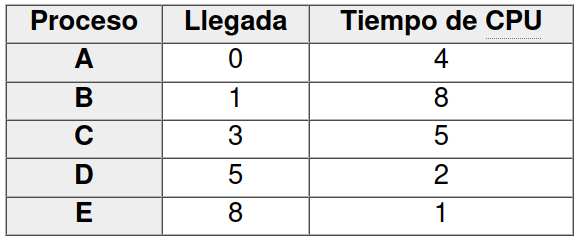
\includegraphics[scale=0.45]{tabla-procesos-orden.png}
        \caption{Tabla de procesos: tiempos de ejecución y llegada}
    \end{figure}

    \item Los procesos se ejecutan en un sistema operativo ideal, es decir, en el que el sistema operativo no consume recursos de CPU.
    \item Comenzamos a estudiar el sistema desde que entran nuestros procesos al sistema y considerando la Unidad de Tiempo 0 (UT0),
    \item En la siguiente tabla se pueden apreciar los procesos que se ejecutan en estas condiciones desde la Unidad de Tiempo 0 (UT0) a la Unidad de Tiempo 1 (UT1).

    \begin{figure}[ht]
        \centering
        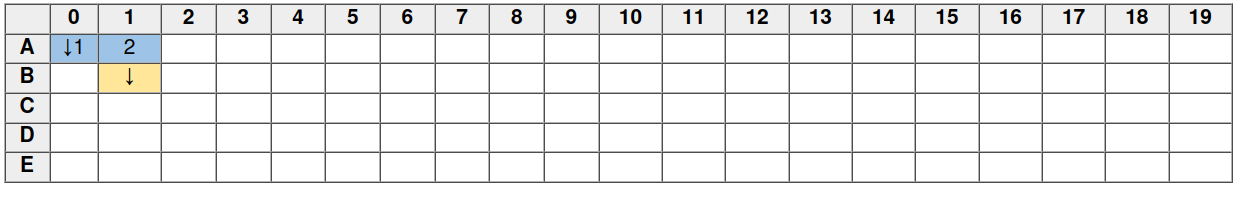
\includegraphics[scale=0.40]{tabla-procesos-gestor.png}
        \caption{Tabla de gestión de los procesos}
    \end{figure}

    \begin{figure}[ht]
        \centering
        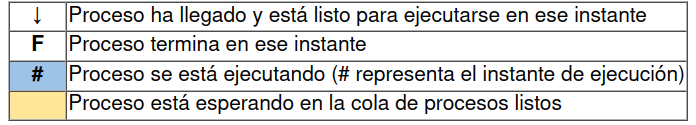
\includegraphics[scale=0.45]{tabla-procesos-leyenda.png}
        \caption{Leyenda de la tabla de gestión de procesos}
    \end{figure}
\end{enumerate}

Respetando todas las restricciones dadas en el enunciado:

\begin{enumerate}
    \item Completa la tabla anterior para las unidades de tiempo de la 2 a la 19, estableciendo el proceso que se ejecutará en cada unidad de tiempo e indicando los instantes de llegada de cada proceso. Utiliza la nomenclatura y/o simbología que aparece en la leyenda.
    \item Razona tu respuesta especificando el estado en el que se encuentra cada uno de los procesos para las unidades de tiempo de la 2 a la 8.
\end{enumerate}

\textbf{Nota:} En el apartado "3.2.- Planificación apropiativa y no apropiativa" de la unidad tienes vídeos con ejemplos resueltos de los principales algoritmos de planificación estudiados.

\subsubsection{Solución}

Hay que tener en cuenta que se esta usando una algoritmo \textbf{SJF} (Short Job First), por lo que los procesos con menos tiempo de ejecución tendrán más prioridad que los que tengan más. Además, es un algoritmo \textbf{no apropiativo}, por lo que una vez que un proceso está ocupando la CPU el sistema operativo no podrá bloquearlo. Teniendo esto en cuenta, vamos a responder a los dos apartados que se nos piden.

\begin{enumerate}
    \item En primer lugar, vamos a mostrar la tabla de ejecución de los procesos. La nomenclatura es la que se especifica en el enunciado por lo que no se va a repetir aquí.

    \begin{figure}[ht]
        \centering
        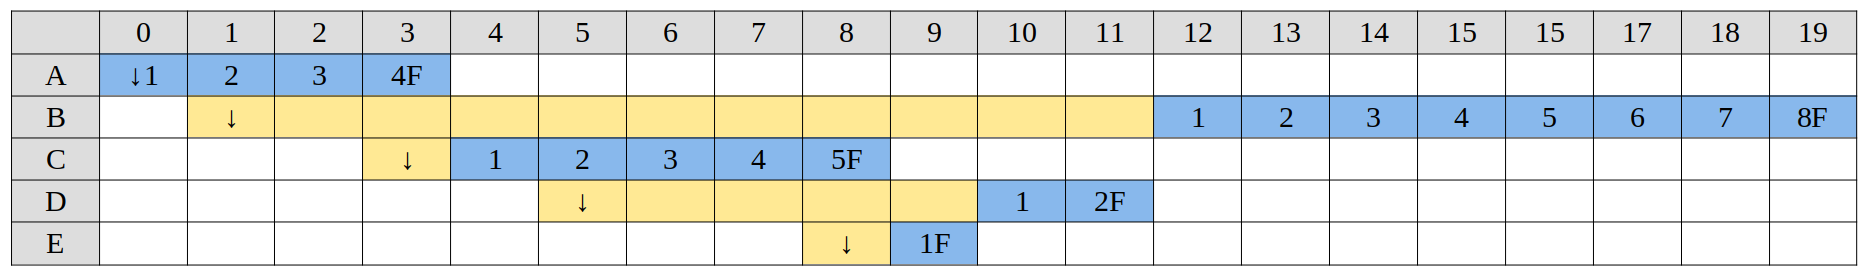
\includegraphics[scale=0.25]{tabla-procesos-solu.png}
        \caption{Tabla de ejecución de procesos resuelta.}
    \end{figure}

    \item Los resultados obtenidos en la tabla se deben, como ya hemos comentado, a que se esta usando un algoritmo SJF, por lo que si en un momento dado hay varios procesos a la espera, siempre tendrá prioridad el que tenga menos ciclos de computación. Ademas, una vez que este proceso ocupa la CPU, no hay forma de bloquearlo, ya que el algoritmos es de tipo \textbf{no apropiativo}. Vamos a analizar con más detalle los momentos de ejecución entre el punto 2 y el 8, incluidos.

    \begin{itemize}
        \item \textbf{Momento 2}: en este momento de la ejecución, tenemos al proceso \textbf{A ejecutándose}, ya que llego en la unidad de tiempo 1, cuando no había ningún proceso más y comenzó a ejecutarse. El proceso \textbf{B} está en \textbf{espera}, ya que llego en el momento 2 cuando ya se estaba ejecutando el proceso A y al ser un algoritmo no apropiativo, el proceso A no se puede bloquear.

        \item \textbf{Momento 3}: en este punto sigue \textbf{ejecutándose} el proceso \textbf{A}, que se encuentra en su último ciclo de computación, y el proceso \textbf{B} sigue en \textbf{espera}, pero además, acaba de entrar el proceso \textbf{C}, que tendrá que ponerse a la espera.

        \item \textbf{Momento 4}: ahora el proceso \textbf{A} ha finalizado y teníamos 2 procesos a la espera, el \textbf{B} y el \textbf{C}. Como estamos usando el algoritmo SJF, se ejecutará el proceso con menos ciclos de computación, por lo que el proceso \textbf{C}, con \textbf{5 ciclos de computación}, tendrá prioridad sobre \textbf{B}, que tiene \textbf{8 ciclos}. Así que el proceso \textbf{C} comenzará su \textbf{ejecución} mientras \textbf{B} sigue a la \textbf{espera}.

        \item \textbf{Momento 5}: el proceso \textbf{C} sigue en \textbf{ejecución}, mientras que el proceso \textbf{B} sigue a la espera y el proceso que acabo de entrar, el \textbf{D}, entrará en \textbf{espera} también.

        \item \textbf{Momento 6}: aquí no ha cambiado nada, seguimos teniendo el mismo estado que en el punto anterior. El único cambio sería que el proceso en ejecución, el \textbf{C}, va por el 3 ciclo de computación.

        \item \textbf{Momento 7}: misma situación que en el punto anterior, ningún cambio salvo un un ciclo más de computación para el proceso \textbf{C}.

        \item \textbf{Momento 8}: en este punto, el proceso \textbf{C} está en su último ciclo de computación. Tenemos a los procesos \textbf{B} y \textbf{D} en espera, además acaba de entrar el proceso \textbf{E}, que pasará a estar a la espera también.  Como ya es el último ciclo de computación de \textbf{C}, habrá que seleccionar el proceso que se ejecutará a continuación. Tenemos 3 procesos a la espera, proceso \textbf{B} con 8 ciclos de computación, el proceso \textbf{D} con 2 ciclos de computación y el proceso que acaba de llegar, el \textbf{E} con 1 ciclo de computación. Como el proceso con menos tiempo de computación es el que tiene prioridad, en el \textbf{siguiente ciclo} se \textbf{ejecutará} el proceso \textbf{E}.
    \end{itemize}
\end{enumerate}

\subsection{Actividad 6: Gestión de Memoria}
Supón un sistema en el que la gestión de memoria se realiza siguiendo un esquema de asignación de particiones variables en el que no es posible realizar compactación de memoria (no se pueden mover de sitio los procesos una vez hayan sido ubicados en memoria). La capacidad de la memoria es de 4000 KB, de los cuales 500 se encuentran ocupados por el sistema operativo, y el resto está disponible para ubicar los procesos que se ejecuten. La situación de partida, la podemos ver en la Figura 2.7.

\newpage

\begin{figure}[ht]
    \centering
    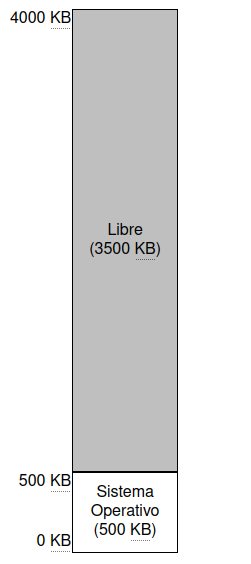
\includegraphics[scale=0.50]{ram-inicial.png}
    \caption{Imagen de la situación inicial de la memoria}
\end{figure}

Se van produciendo las siguientes llegadas y salidas de procesos, por orden, que requieren la asignación o liberación de trozos de memoria:

\begin{enumerate}
    \item Inicialmente solo está cargado el sistema operativo, sin ningún otro proceso (situación de partida).
    \item Llega un proceso A de 1200 KB de tamaño y se intenta cargar en memoria.
    \item Llega un proceso B de 500 KB de tamaño y se intenta cargar en memoria.
    \item Llega un proceso C de 1000 KB de tamaño y se intenta cargar en memoria.
    \item Llega un proceso D de 400 KB de tamaño y se intenta cargar en memoria.
    \item El proceso B termina su ejecución y se libera el espacio que estaba ocupando en memoria.
    \item Llega un proceso E de 600 KB de tamaño y se intenta cargar en memoria.
\end{enumerate}

Realiza lo siguiente:

\begin{enumerate}[label=(\alph*)]
    \item Si consideramos que el dibujo de arriba se corresponde con el punto 1 de la lista anterior, incluye dos dibujos más en los que se muestre cómo se encontraría la memoria después de los instantes 5 (tras llegar D y cargarse en memoria) y 6 (tras terminar B y liberarse su espacio).
    \item Explica qué ocurre en el punto 7, cuando llega E e intenta cargarse en memoria. Comenta si ocurre algún tipo de fragmentación y, en caso afirmativo, qué tipo de fragmentación sería.
\end{enumerate}

\subsubsection{Solución}
En este punto vamos a ver como se gestionaría la memoria en un sistema operativo con esquema de asignación de particiones variables en el que no es posible la compactación, que como veremos a continuación, provocara la fragmentación de la memoria.

\begin{enumerate}[label=(\alph*)]
    \item En primer lugar, vamos a ver como quedaría la memoria en los instantes 5 y 6. El espacio en gris representa la memoria libre, y como podemos ver, tras el paso 6, quedan dos espacios de memoria libres de 400 y 500 KB.
    \begin{figure}[ht]
        \centering
        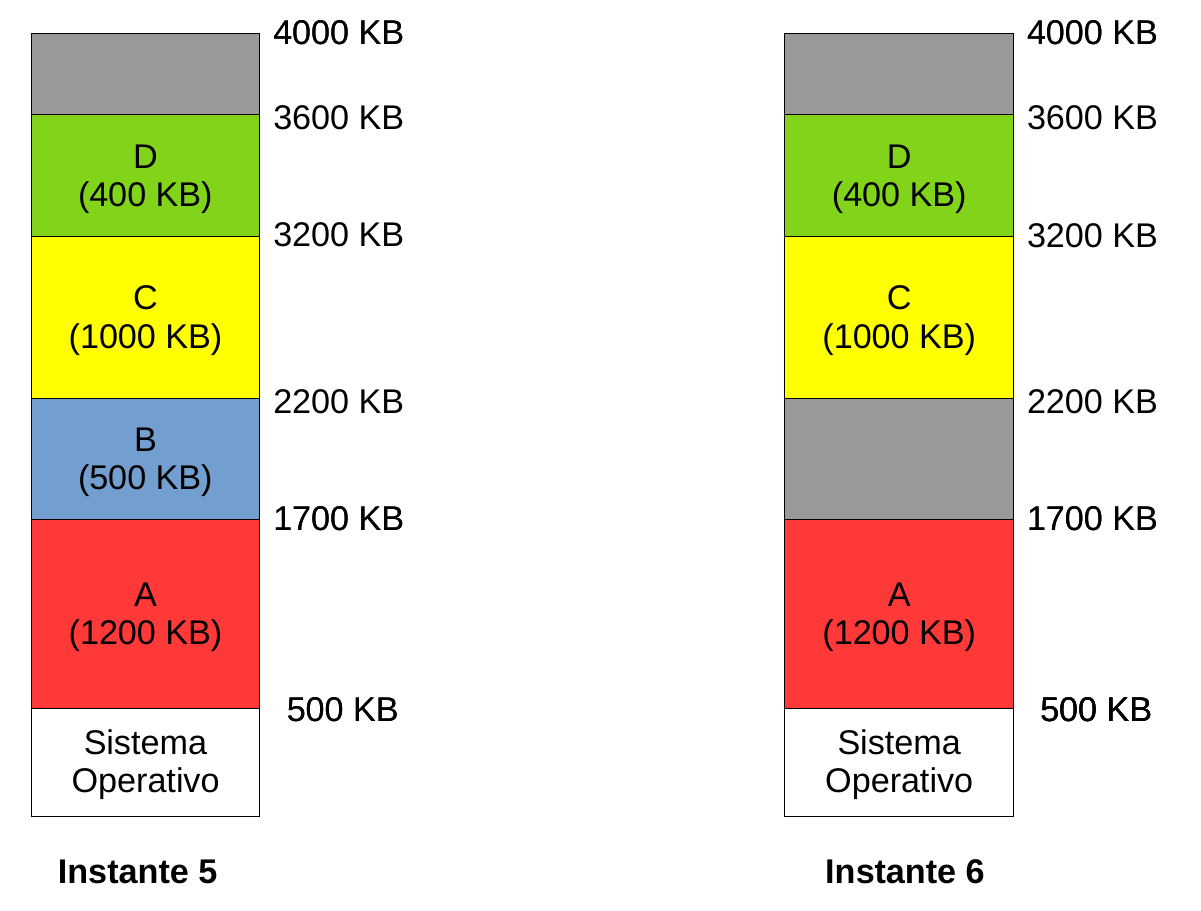
\includegraphics[scale=0.25]{ram-final.png}
        \caption{Estado de la memoria en los pasos 5 y 6}
    \end{figure}
    \item Al entrar un proceso \textbf{E} de \textbf{600 KB}, no podría cargarse en memoria, ya que los espacios libres, como he comentado en el punto anterior, son de \textbf{400 KB} y \textbf{500 KB}. Esto provocaría un estado de \textbf{fragmentación externa} en la memoria, ya que la memoria externa a las particiones no es lo suficientemente grande como para alojar al nuevo proceso, por lo que en es punto, y hasta que algún proceso liberara memoria, no se podría usar.
\end{enumerate}

\subsection{Actividad 7: Estructura de Directorios y Rutas}
Considera las siguientes estructuras de directorios para un equipo con SO Windows 10 (A) y uno con SO Lubuntu 22.04 (B):

\begin{figure}[ht]
    \centering
    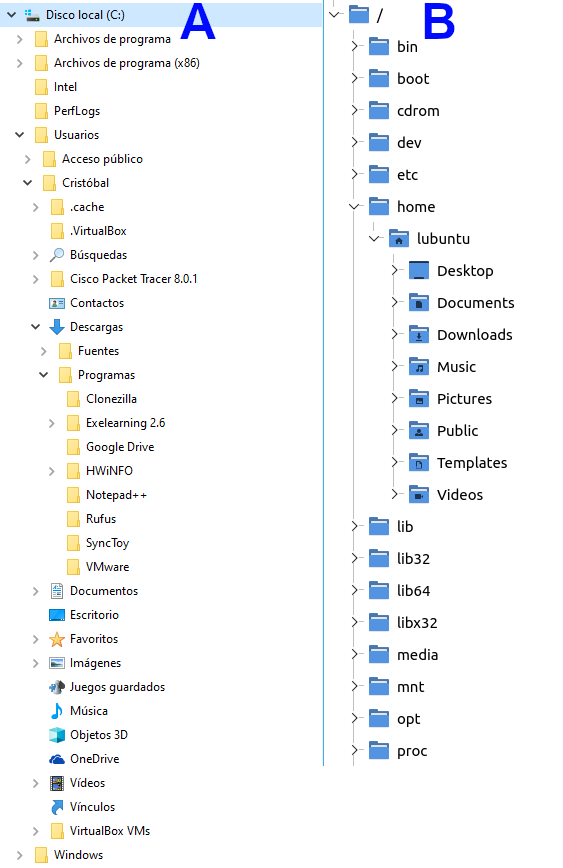
\includegraphics[scale=0.35]{estructura-directorios.png}
    \caption{Estructuras de directorios para Windows y Lubuntu}
\end{figure}

Para el equipo con Windows (A), escribe las siguientes rutas:

\begin{itemize}
    \item Una ruta absoluta al directorio "Fuentes".
    \item Una ruta relativa al directorio "Rufus", considerando que el directorio de trabajo/activo actual sea "Imágenes".
    \item \textbf{NOTA:} Las rutas en Windows no son sensibles a mayúsculas y minúsculas.
\end{itemize}

Para el equipo con Linux (B), escribe las siguientes rutas:

\begin{itemize}
    \item Una ruta absoluta al directorio "Downloads".
    \item Una ruta relativa al directorio "Pictures", considerando que el directorio de trabajo/activo actual sea "media".
    \item \textbf{NOTA:} Las rutas en Linux sí son sensibles a mayúsculas y minúsculas.
\end{itemize}

\subsubsection{Solución}

\begin{enumerate}[label=(\alph*).]
    \item Rutas para \textbf{Windows}
    \begin{itemize}
        \item \textbf{Ruta Absoluta} a ``Fuentes'':
        \begin{figure}[h]
                \begin{verbatim}
        C:\Usuarios\Cristóbal\Descargas\Fuentes\
                \end{verbatim}
        \end{figure}

         \item \textbf{Ruta Relativa} a ``Rufus'' desde el directorio ``Imágenes'':
            \begin{figure}[h]
                \begin{verbatim}
        ..\Usuarios\Cristóbal\Descargas\Programas\Rufus\
                \end{verbatim}
            \end{figure}
    \end{itemize}

    \item Rutas para \textbf{Lubuntu}:
    \begin{itemize}
        \item \textbf{Ruta Absoluta} a ``Downloads'':
        \begin{figure}[h]
            \begin{verbatim}
        /home/lubuntu/Downloads/
            \end{verbatim}
        \end{figure}

        \item \textbf{Ruta Relativa} a ``Pictures'' desde el directorio ``media'':
        \begin{figure}[H]
            \begin{verbatim}
        ../home/lubuntu/Pictures
            \end{verbatim}
        \end{figure}
    \end{itemize}
\end{enumerate}
% Bibliography

\newpage
\bibliography{citas}
\bibliographystyle{unsrt}

\end{document}